\chapter{Umsetzung eines Testprojektes mit Rayden}
\label{cha:Testen}

In diesem Kapitel wird ein Testprojekt mit dem Rayden-System umgesetzt. Dazu wird gezeigt, wie man unterschiedliche Testmethode mit dem Rayden-System verwenden kann. Um sinnvolle Tests schreiben zu können wird eine Beispielanwendung benötigt, welche in Abschnitt \ref{cha:demoapp} beschrieben wird. In den nächsten drei Abschnitten \ref{cha:TestenUnit}, \ref{cha:TestenApi} und \ref{cha:TestenUA} wird die Umsetzung von unterschiedlichen Testmethoden mit den Rayden-System gezeigt. Ein besonders Augenmerk wurde dabei auf die Abnahmetests gelegt.

%%------------------------------------------------------------------------------------------------------

\section{Beispielanwendung}
\label{cha:demoapp}

Für das Evaluieren des Rayden-Systems wird eine Anwendung zum Test benötigt. Bei der Anwendung sollte es sich um eine Webanwendung handeln, um die Unterstützung von Selenium zeigen zu können. Für die Evaluierung hat man sich für die \enword{PetClinic}-Webanwendung entschieden, welche eine Beispielanwendung des Spring-Projekts ist. Die Anwendung mit allen Ressourcen ist öffentlich auf Github unter der Adresse \enword{https://github.com/spring-projects/spring-petclinic/} zugänglich.

\begin{figure}
\centering
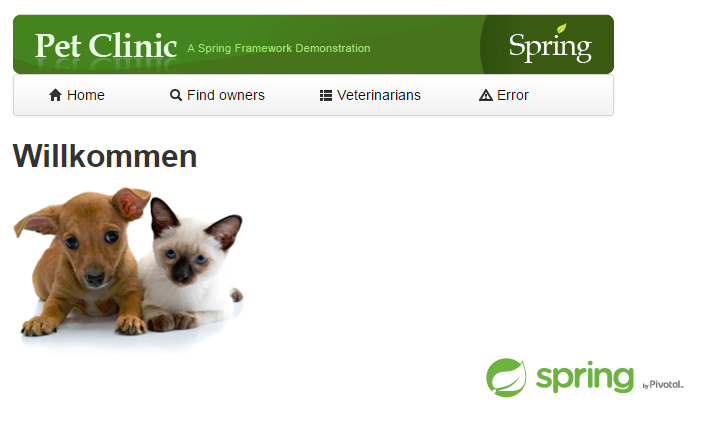
\includegraphics[width=0.9\textwidth]{petclinic.png}
\caption{Startseite der Webanwendung PetClinic}
\label{fig:petClinicPage}
\end{figure}

\SuperPar
Bei der \enword{PetClinic}-Anwendung handelt es sich um eine Verwaltungssoftware für eine Tierklinik. Mit der Anwendung können Besuche bei einem Tierarzt protokolliert werden. Dazu gehört die Erfassung der Tierbesitzer mit ihren Haustieren. Zu jedem Haustier werden alle Arztbesuche gespeichert, damit der Krankheitsverlauf dokumentiert ist. Neben den Besitzer und ihren Tieren werden Tierärztinnen und Tierärzte verwaltet. 

\SuperPar
Da der Funktionsumfang der Anwendung überschaubar ist, eignet sich diese ausgezeichnet als Beispielanwendung für die Evaluierung des Rayden-System. In den nächsten Abschnitten werden Test mit unterschiedlichen Testmethoden für die \enword{PetClinic}-Anwendung gezeigt.

\SuperPar
In den folgenden Abschnitte \ref{cha:TestenUnit}, \ref{cha:TestenApi} und \ref{cha:TestenUA} werden Tests für die \enword{Petclinic}-Anwendung vorgestellt. Diese Tests wurden mit drei unterschiedlichen Testmethoden umgesetzt um zu zeigen, wie man die Testmethoden mit dem Rayden-System vereinen kann.

%%------------------------------------------------------------------------------------------------------
\section{Komponententests}
\label{cha:TestenUnit}

Dieser Abschnitt zeigt die Umsetzung eines Komponententests mit dem Rayden-System. Für einen Komponententest wir in Rayden zuerst ein \enword{Keyword} angelegt. Der Codeauszug \ref{prog:unitTest} zeigt die Definition des \enword{Keywords}. Ein Komponententest wird normalerweise als \enword{Scripted-Keyword} umgesetzt und mit dem \enword{Keyword}-Typ \enword{unittest} gekennzeichnet. In diesem Beispiel wird die Komponente \enword{PetTypeFormatter} getestet. Die Komponente ist in der Webanwendung dafür verantwortlich, aus einer Zeichenkette das dazugehörige Domänenobjekt zu liefern und umgekehrt. 

\begin{program}
\begin{JavaCode}
unittest Test PetTypeFormatter {
	''' This unittest verifies the functionality of the 
	    formatter class PetTypeFormatter '''
	implemented in java -> "petclinic.TestPetTypeFormatterKeyword"
}
\end{JavaCode}
\caption{Komponententest \enword{Test PetTypeFormatter}}
\label{prog:unitTest}
\end{program}

\SuperPar
Der Codeausschnitt \ref{prog:unitTestImpl} zeigt die Implementierung des \enword{Scripted-Keywords}. Die Implementierung des Komponententests ist grundlegend gleich mit einem normalen JUnit-Test. Die großen Unterschiede sind, dass die Methode nicht mit \enword{@Test} annotiert werden und dass es nur eine Testmethode pro Klasse geben kann. 

\begin{program}
\begin{JavaCode}
public class TestPetTypeFormatterKeyword implements ScriptedKeyword {

  @Override
  public KeywordResult execute(String keyword, KeywordScope scope, RaydenReporter reporter) {
    ClinicService service = new MockClinicService();
    PetTypeFormatter formatter = new PetTypeFormatter(service);

    try {
     Assert.assertEquals("dog", formatter.parse("dog", null).getName());
     Assert.assertEquals("cat", formatter.parse("cat", null).getName());
     Assert.assertEquals("fish",formatter.parse("fish",null).getName());
    } catch (ParseException e) {
      throw new AssertionError(e);
    }
    
    try {
      formatter.parse("hamster", null);
      Assert.fail("No ParseExeption was thrown!");
    } catch (ParseException e) {
    }

    try {
      formatter.parse(null, null);
      Assert.fail("No ParseExeption was thrown!");
    } catch (ParseException e) {
    }

    return new KeywordResult(true);
  }
}
\end{JavaCode}
\caption{Implementierung des \enword{Test PetTypeFormatter} \enword{Keywords}}
\label{prog:unitTestImpl}
\end{program}

\SuperPar
Eine nützliche Erweiterung des Rayden-Systems in der Zukunft wäre eine bessere Integration mit \enword{Unittest-Frameworks} wie JUnit oder TestNG.

%%------------------------------------------------------------------------------------------------------
\section{Schnittstellentest}
\label{cha:TestenApi}

Bei einem Schnittstellentest werden öffentliche Schnittstellen wie ein \enword{Restful}-Schnittstelle \cite{Rest} getestet. Im Schnittstellentest \ref{prog:integrationTest} wird die \enword{Restful}-Schnittstelle für Tierärzte getestet. Schnittstellentests können entweder als \enword{Compound-Keywords} oder als \enword{Scripted-Keywords} definiert werden. Es hängt ganz davon ab, ob die Implementierung des \enword{Scripted-Keywords} in einem anderen Test wieder verwendet werden kann. 

\begin{program}
\begin{JavaCode}
apitest Test Veterinarians Restful Service {
	'''This keyword checks the restfull service for veterinarian.'''
	
	Verify Json("http://localhost:9966/petclinic/vets.json", 
	            "./demodata/vets.json")
}

keyword Verify Json {
  '''The keyword download the content from the given url. A second 
	   content is loaded from the file. The both contents are parsed
		 into a JSON object tree. If the two trees were equals, the 
		 keyword finish successfully'''
		
	parameter url
	parameter file

	implemented in java -> "petclinic.VerifyJsonKeyword"
}
\end{JavaCode}
\caption{Integrationstest \enword{Test Veterinarians Restful Service}}
\label{prog:integrationTest}
\end{program}

\SuperPar 
Bei diesen Beispiel liefert die Schnittstelle das Ergebnis als einen JSON-Text. Um zu Überprüfen ob die Schnittstelle korrekt funktioniert, wird dieser Text mit einem Text aus einer Demodaten-Datei verglichen. Damit der Test erfolgreich durchläuft, müssen die beiden Texte semantisch Gleich sein. Semantisch Gleich heißt bei einem JSON-Text, dass die enthaltenen Daten gleich sein müssen, aber nicht in welcher Reihenfolge diese serialisiert worden sind.

\begin{program}
\begin{JavaCode}
public class VerifyJsonKeyword implements ScriptedKeyword {
  @Override
  public KeywordResult execute(String keyword, KeywordScope scope, RaydenReporter reporter) {
    String url = scope.getVariableAsString("url");
    String file = scope.getVariableAsString("file");

    try {
      CloseableHttpClient client = HttpClientBuilder.create().build();
      CloseableHttpResponse response = client.execute(new HttpGet(url));
      if (response.getStatusLine().getStatusCode() != 200) {
        return new KeywordResult(false);
      }
      String json = IOUtils.toString(response.getEntity().getContent());

      JsonParser parser = new JsonParser();
      JsonElement o1 = parser.parse(json);
      JsonElement o2 = parser.parse(IOUtils.toString(new FileInputStream(file)));

      return new KeywordResult(o1.equals(o2));
    } catch (IOException e) {
      throw new RuntimeException(e);
    }
  }
}
\end{JavaCode}
\caption{Implementierung des \enword{Verify Json Keywords}}
\label{prog:integrationTestImpl}
\end{program}

\SuperPar
Wenn mehrere Schnittstellen dieser Art getestet werden, ist es sinnvoll, dass man die Funktionalität zum Abfragen und Vergleichen der Daten in ein separates \enword{Keyword} kapselt. Dadurch können andere Tests dieses \enword{Keyword} wiederverwenden. Die Implementierung des \enword{Verify Json Keywords} zeigt das Codebeispiel \ref{prog:integrationTestImpl}. Das Codestück zeigt, dass zuerst über einen \enword{HttpClient} der JSON-Text von einem Server abgefragt wird. Danach wird der JSON-Text mit einem \enword{Parser} in einem Objektbaum transformiert. Dafür wird eine \enword{Parser}-Implementierung aus der \enword{Google-Guava}-Bibliothek verwendet. Der selbe Prozess wird auch mit der Demodaten-Datei durchlaufen. Am Ende gibt es zwei Objektbäume für die JSON-Texte. Für den semantischen Vergleich der beiden Bäume kann die Methode \enword{equals()} der Klasse \enword{JsonElement} verwendet werden. Diese Klasse stammt wiederum aus der \enword{Google-Guava}-Bibliothek.

%%------------------------------------------------------------------------------------------------------
\section{Abnahmetests}
\label{cha:TestenUA}

In diesem Abschnitt wird die letzte Testmethode für die Evaluierung erläutert. Dabei handelt es sich um Abnahmetests, die wohl wichtigste Testmethode für das Rayden-System. Ein Großteil des Rayden-System ist primär für die Unterstützung dieser Testmethode entwickelt worden. Aus diesem Grund enthält dieser Abschnitt auch zwei Umsetzungen von Testmethoden mit Rayden. Als erstes wird der Testfall \enword{Suchen nach einen Tierbesitzer} \ref{cha:TestenUA1} umgesetzt. Bei diesem Testfall wird die Suche der \enword{Petclinic}-Anwendung getestet. Im zweiten Testfall \ref{cha:TestenUA2} wird das Anlegen eines neuen Tierbesitzers gezeigt. 

\SuperPar
Für das Steuern der Browser wurde für beide Abnahmetests die Selenium-Bibliothek verwendet. Aus diesem Grund wird im dritten Teil \ref{cha:TestenSelenium} dieses Abschnittes die Bindung zwischen dem Rayden-System und der Selenium-Bibliothek gezeigt. 

%%------------------------------------------------------------------------------------------------------

\subsection{Abnametest \enword{Suchen nach einen Tierbesitzer}}
\label{cha:TestenUA1}

Bei dem  Abnahmetest im Codeausschnitt \ref{prog:uatest-find} wird die Suchfunktion der \enword{Petclinic}-Anwendung getestet. Dafür wird der Testfall als erstes in zwei \enword{Compound-Keywords} \enword{Find a specific Pet Owner} und \enword{Check Owner Details} aufgeteilt. Neben den beiden \enword{Keywords} werden noch zwei weiter \enword{Keywords} \enword{Prepare Browser} und \enword{Cleanup Browser}  benötigt, welche für das Starten und Stoppen des Browsers zuständig sind. 

\begin{program}
\lstinputlisting{samplecode/uatest-findpetowner.rlg}
\caption{Abnametests: \enword{Suchen nach einen Tierbesitzer}}
\label{prog:uatest-find}
\end{program}


\begin{program}
\lstinputlisting{samplecode/or-findpetowner.rlg}
\caption{Codeauszug aus dem \enword{Object Repository} für den Testfall \enword{Suchen nach einen Tierbesitzer}}
\label{prog:or-find}
\end{program}

\SuperPar
Das \enword{Keyword} \enword{Find a specific Pet Owner} führt die Suche nach einem Tierbesitzer mit dem Name \enword{Davis} aus. Dafür navigiert das \enword{Keyword} auf die Seite für Tierbesitzer und startet die Suche nach allen Besitzern. Danach werden auf der Ergebnisseite der Suche alle Besitzer aufgelistet, welche in der Anwendung vorhanden sind. Danach wird mithilfe der integrierten Suche nach dem Namen \enword{Davis} gesucht und die Detailseite des Tierbesitzers geöffnet. Wurde die Detailseite erfolgreich geöffnet ist das \enword{Keyword} am Ende. Die Validierung der Daten werden von dem nächsten \enword{Keyword} \enword{Check Owner Details} durchgeführt.

\SuperPar
Dem \enword{Keyword} \enword{Check Owner Details} werden die zu überprüfenden Daten als Parameter übergeben. Das \enword{Keyword} überprüft jedes Datum mit dem \enword{Scripted-Keyword} \enword{Verify Text}. Dem \enword{Scripted-Keyword} werden zwei Parameter übergeben. Der erste Parameter ist ein \enword{Locator}, welcher ein Element auf der Webseite definiert. Von diesem Element wird der Text abgefragt und mit dem zweiten Parameter verglichen. Der zweite Parameter ist eine Zeichenkette mit dem erwarteten Wert. Sind die Wert nicht gleich, wird der Test mit einem Fehler abgebrochen. 

\begin{figure}
\centering
\includegraphics[width=1\textwidth]{or.png}
\caption{Darstellung der Verbindung von Objekt aus dem \enword{Objekt-Repository} mit Elementen auf der Webseite}
\label{fig:orwebsite}
\end{figure}

\SuperPar
Damit in den \enword{Keywords} keine \enword{XPath}-Ausdrücke vorkommen müssen, wird ein \enword{Objekt-Repository} verwendet. Einen Auszug mit den wichtigsten Objekten für diesen Abnahmetest zeigt das Codebeispiel \ref{prog:or-find}. Das Codebeispiel enthält die Objekte für die Suchergebnisseite und die Detailseite für Tierbesitzerinnen und Tierbesitzer. Die Abbildung \ref{fig:orwebsite} zeigt die Abbildung von Webseiten-Element auf Objekt im \enword{Objekt-Repository}. In der Grafik sind jene Element rot hinterlegt, welche ein Eintrag im \enword{Objekt-Repository} besitzen. Neben jeden Element steht auch der vollständige \enword{Locator}, mit welchem man das Objekt aus \enword{Objekt-Repository} abfragen kann.

%%------------------------------------------------------------------------------------------------------

\subsection{Abnametest \enword{Anlegen eines neuen Tierbesitzer}}
\label{cha:TestenUA2}


Der zweite Abnahmetest testet den Anwendungsfall \enword{Anlegen eines neuen Tierbesitzer}. Diese Abnahmetest wird direkt im Abnahmetest-\enword{Keyword} aus spezifiziert. Als erstes wird wiederum die Testumgebung mit dem \enword{Keyword} {Preapre Browser} vorbereitet. Im nächsten Schritt navigiert der Test auf die Tierbesitzerseite und klick auf die \enword{Add Owner} Schlatfläche. 


\SuperPar
Danach werden alle benötigten Daten für eine neue Tierbesitzerin oder Tierbesitzer im Formular eingegeben. Dazu wird das \enword{Keyword} \enword{Type Text} verwendet. Diese \enword{Scripted-Keyword} schreibt mithilfe der Selenium-Bibliothek einen Text in ein Textfeld auf der Webseite. Der Codeauszug \ref{prog:or-create} zeigt die dazugehörige Objekt im \enword{Object Repository}.  Der Auszug zeigt die Seite \enword{Edit Owner Page}, welche das Formular für das Anlegen und Änderen einer Besitzerin oder eines Besitzers zeigt.

\SuperPar
Das \enword{Add new pet owner} \enword{Keyword} ist ein gutes Beispiel, um zu zeigen, wie man mithilfe des \enword{Object Repository} einen leserlichen Test schreiben kann. Der Test setzt auschließlich auf \enword{Locators}  und verzeicht auf die direkte Verwendung von \enword{XPath}-Ausdrücken. 

\begin{program}
\lstinputlisting{samplecode/or-createpetowner.rlg}
\caption{Codeauszug aus dem \enword{Object Repository} für den Testfall \enword{Anlegen eines neuen Tierbesitzer}}
\label{prog:or-create}
\end{program}

%%------------------------------------------------------------------------------------------------------

\subsection{\enword{Keywords} aus der Selenium-Bibliothek}
\label{cha:TestenSelenium}

In diesem Abschnitt werden ausgewählte Selenium \enword{Keywords} aus den Abhnametests beschrieben. Diese \enword{Keywords} wurden alle in der Datei \enword{selenium.rlg} angelegt. Die Datei \enword{selenium.rlg} stellt somit die \enword{Bridge} zwischen Rayden und Selenium dar. Das Codestück \ref{prog:selenium} zeigt drei \enword{Scripted-Keywords}, welche einen guten Überblick in die Integration von Selenium in das Rayden-System zeigen. 

\begin{program}
\lstinputlisting{samplecode/selenium.rlg}
\caption{Codeauszug aus der Selenium \enword{Keyword}-Bibliothek}
\label{prog:selenium}
\end{program}

\SuperPar
Als erstes wird das \enword{Open Browser Keyword} \ref{prog:openBrowserKeyword} beschrieben. Dieses \enword{Scripted-Keyword} ist essentiel für die Verwendung von Selenium, da dieses \enword{Keyword} die Testumgebung vorbereit. Als Parameter werden der Browsertyp und eine \enword{URL} übergeben. Der Browsertyp definiert den Browser, welcher gestartet werden soll. Das kann zum Beispiel der \enword{Internet Explorer}, \enword{Firefox} oder \enword{Google Chrome} sein. Mit dem Browsertyp Parameter wird eine \enword{Webdriver}-Objekt angelegt. Dieses Objekt dient als Schnittstelle zwischen dem Test und Browser-Instanz. Jedes neue \enword{Webdriver}-Objekt startet einen Browser. Der zweite Parameter \enword{URL} definiert die Startseite. Über die Methode \enword{navigate()} der Klasse \enword{Webdriver} kann man auf eine neue Seite im Browser navigieren. 

\begin{program}
\begin{JavaCode}
public class OpenBrowserKeyword implements ScriptedKeyword {

	@Override
	public KeywordResult execute(String keyword, KeywordScope scope, RaydenReporter reporter) {
		String browserType = scope.getVariableAsString("browserType");
		String url = scope.getVariableAsString("url");
		WebDriver driver = Selenium.getInstance().initializeDriver(browserType);
		driver.navigate().to(url);
		return new KeywordResult(true);
	}
}
\end{JavaCode}
\caption{Implementierung des \enword{Open Browser Keywords}}
\label{prog:openBrowserKeyword}
\end{program}

\SuperPar
Bei dem nächsten \enword{Keyword} handelt es sich um das \enword{Click Keyword}, welches im Codestück \ref{prog:clickKeyword} gezeigt wird. Mit diesem \enword{Keyword} kann man einen Klick auf der Webseite auslösen. Um die richtige Position für den Klick herausfinden zu können, wird dem \enword{Keyword} ein \enword{Locator} übergeben. Dieser \enword{Locator} beschreibt ein Element auf der Webseite. Die Auswertung dieses \enword{Locators} wird von der Methode \enword{findElement()} übernommen. Die Methode greift auf das aktuelle \enword{WebDriver}-Objekt zu um das Element zu finden. Diese Aktion könnte man auch direkt über das \enword{WebDriver}-Objekt ausführen, jedoch enthält die Methode \enword{findElement()} aus der Selenium Klasse einen zusätzlichen Wiederholungsfunktion im Fehlerfall. Die Funktionalität ist für einen stabilen Abnahmetest wichtig, da dieses Synchronisierungsprobleme mit der Webanwendung reduziert. 

\begin{program}
\begin{JavaCode}
public class ClickKeyword implements ScriptedKeyword {

  @Override
  public KeywordResult execute(String keyword, KeywordScope scope, RaydenReporter reporter) {
    RaydenExpressionLocator locator = (RaydenExpressionLocator) scope.getVariable("locator");
    reporter.log("Click on '" + locator + "'");
    Selenium.getInstance().findElement(locator.getEvalLocator()).click();
    return new KeywordResult(true);
  }
}
\end{JavaCode}
\caption{Implementierung des \enword{Click Keywords}}
\label{prog:clickKeyword}
\end{program}

\SuperPar
Man spricht von einem Synchronisierungsfehler bei einer Webseite, wenn eine Aktion ausgeführt wird, obwohl die Anwendung noch nicht fertig geladen ist. Dieser Fehler tritt sehr häufig bei stark dynamischen Webseiten auf. Die einfachste und auch primitivste Lösung für das Problem ist die mehrmalige Auswertung des \enword{XPath}-Ausdruckes, falls dieser kein Element findet. Genau dieser Ansatz ist in der \enword{findElement()} Methode der Selenium Klasse implementiert.

\begin{program}
\begin{JavaCode}
public class VerifyTextKeyword implements ScriptedKeyword {

  @Override
  public KeywordResult execute(String keyword, KeywordScope scope, RaydenReporter reporter) {
    RaydenExpressionLocator locator = (RaydenExpressionLocator) scope.getVariable("locator");
    String text = scope.getVariableAsString("text");
    WebElement element = Selenium.getInstance().findElement(locator.getEvalLocator());
    String elementText = element.getText();
    reporter.log("Verify Text: '" + text + "'='" + elementText + "'");
    return new KeywordResult(text.equals(elementText));
  }
}
\end{JavaCode}
\caption{Implementierung des \enword{Verify Text Keywords}}
\label{prog:verifyTextKeyword}
\end{program}

\SuperPar
Bei dem \enword{Keyword} \enword{Verify Text} handelt es sich um eine Verifikation. Mit diesem \enword{Keyword} kann ein Text auf einer Webseite mit einer vordefinierten Text verglichen werden. Bei einem Fehlerfall wird das \enword{Keyword} mit einem Fehler beendet und die Ausführung des Tests abgebrochen. Die Implementierung des \enword{Scripted-Keywords} zeigt der Codeausschnitt \ref{prog:verifyTextKeyword}. Das Ergebnis des Vergleichs der beiden Text wird an ein \enword{KeywordResult}-Objekt übergeben. 


\section{Testdokumentation}

\todo
Vielleicht löschen?

\SuperPar
Diese Kapitel hat gezeigt, wie man ein Testprojekt mit Rayden umsetzten kann. Es wurden dafür drei unterschiedliche Testmethode gezeigt und wie diese mit Rayden umgesetzt werden können. Die Tests haben auch gezeigt, welche Vorteil die Verwendung des \enword{Object Repository} hat. Das nächste Kapitel beinhaltet eine Zusammenfassung dieser Masterarbeit und gibt einen Ausblick auf mögliche Erweiterungen des Rayden-Systems. 